\documentclass[a4paper,man,natbib]{apa6}

\usepackage[english]{babel}
\usepackage[utf8x]{inputenc}
\usepackage{amsmath}
\usepackage{graphicx}
\usepackage[colorinlistoftodos]{todonotes}
\usepackage{xcolor}
\usepackage[draft,inline,nomargin,index]{fixme}

\fxsetup{theme=color,mode=multiuser}
\FXRegisterAuthor{ab}{sab}{\color{blue}Amelie} % abnote{} with text inside to edit
\FXRegisterAuthor{bb}{sbb}{\color{purple}Brice} % bbnote{} with text inside to edit
\FXRegisterAuthor{ln}{sln}{\color{violet}Lad} % lnnote{} with text inside to edit

\title{Potential Biasedness of the Sequential Testing Procedure} % ché
\shorttitle{Blind Bayes Factor}
\threeauthors{Amélie G. Bret}{Brice Beffara}{Ladislas Nalborczyk}
\threeaffiliations{Univ. Grenoble Alpes, CNRS, LPNC UMR 5105, F-38000, Grenoble \\Psychological Science Research Institute, Catholic University of Louvain, Belgium}{The Walden III Slowpen Science Laboratory, France}{Univ. Grenoble Alpes, CNRS, LPNC UMR 5105, F-38000, Grenoble \\ Department of Experimental Clinical and Health Psychology, Ghent University}

\abstract{When collecting data, bayesian hypothesis testing allows optional stopping with unlimited multiple testing. This procedure is called Sequential Bayes Factors (SBF). Bayes factors are
computed until an a priori defined level of evidence is reached. This allows flexible sampling plans and
is not dependent upon correct effect size guesses in an a priori power analysis. Testing mean differences between 2 groups, the SBF design typically needs 50\% to 70\% smaller samples to reach a conclusion
about the presence of an effect,  as compared
with optimal NHST, while having the same or lower long-term rate of wrong inference. \todo[inline, color=red]{Le début de l'asbtract est extrait de pain joli et al. Il faudra le reformuler.}}

\begin{document}
\maketitle

\section{Introduction}

\lnnote{Où publier ? S'il s'agit d'un commentaire, il doit être publié dans la même revue que l'article original. Il y a deux papiers qui présentent la méthode SBF, un dans Psych. Meth (2017) et l'autre dans PBR (in press). \newline PBR accepte les commentaires : "Commentaries on previously published articles also appear in the journal...": http://www.springer.com/psychology/cognitive+psychology/journal/13423/PS2?detailsPage=aboutThis \newline Je ne sais pas si Psych. Meth les accepte...}

\bbnote{Exact mais Psych Meth accepte aussi des tuto donc on pourrait peut-être faire passer ça comme un tuto non ?}

\lnnote{Ça me semble un peu léger pour un tuto... non ? On présenterait quoi ? juste une fonction qui ajoute un argument "blind" aux fonctions existantes ? Ça ferait un bon article de blog mais je pense que c'est un peu léger pour un tuto...PS: je pense que Psych. Meth. accepte les comments, même s'ils ne le précisent, mais il faudrait juste s'en assurer... je peux m'occupper de vérifier ça}

\section{Proposition de plan}
\lnnote{
1. Introduction, état du problème
1.1 Présentation de la méthode de sequential testing, telle qu'exposée dans les deux papiers de Schönbrodt et al. (2017a, 2017b)
1.2 Problèmes
1.2.1 Non-respect de l'hypothèse d'indépendance des observations ? Vérifier que c'est un problème pour le BF, mais il me semble que oui...
1.2.2 Biais de demande...sachant la taille d'effet (à trouver) habituelle du biais de demande, on pourrait estimer le biais (i.e., la différence de N entre une procédure de sequential testing non biaisée (i.e., en aveugle) et une procédure biaisée) lié à la connaissance des résultats du participant N-1...
2. Solutions, comment régler le problème ?
2.1 Blinding: soit l'analyste et l'expérimentateur sont deux personnes différentes, soit il s'agit de la même personne mais elle doit se rendre aveugle aux résultats du participant N-1.
2.2 On pourrait aussi proposer une solution pratique immédiate, genre script qui permet de se rendre aveugle aux résultats précédents (j'ai déjà un truc du genre de prêt), voire même un petit package ?}
\bbnote{exact et ça peut donc passer pour un tuto éventuellement}
\lnnote{3. Evaluation du biais ?
3.1 Propositions de protocoles expérimentaux permettant de mettre en évidence le biais.
3.2 On pourrait profiter de ce papier pour lancer un appel à contribution à une grosse manip multi-lab all around the world, pour évaluer l'amplitude de ce biais, comme on avait commencé à discuter...non ?}\bbnote{super idée j'aime cet séquence évolutive vmvc}

\section{Sondage et liste des arguments pour ou contre inclure Wagenmakers, Schönbrodt, Perugini et cie ?}

Pour: ils sont forts, ils peuvent nous éviter de dire des bêtises, ça fait moins "attaque" s'ils sont aussi auteurs...	

Contre: on peut les avoir en reviewers... et ça fait une diversité de point de vues dans la littérature (genre moins crew)

\section{TODO}

...insérer un diagramme qui représente le processus de sequential testing et là où opère notre biais potentiel, si expé = analyste...

...insérer diagramme de nos prédictions...

...finaliser la fonction blind (en cours)...

%...(private) repo github synchronised with Overleaf: \href{https://github.com/lnalborczyk/Blind_BF}{github}

\section{Latex examples}

LaTeX automatically generates a bibliography in the APA style from your .bib file. The citep command generates a formatted citation in parentheses \citep{Lamport1986}. The cite command generates one without parentheses. LaTeX was first discovered by \cite{Lamport1986}.

% Commands to include a figure:
%\begin{figure}
%\centering
%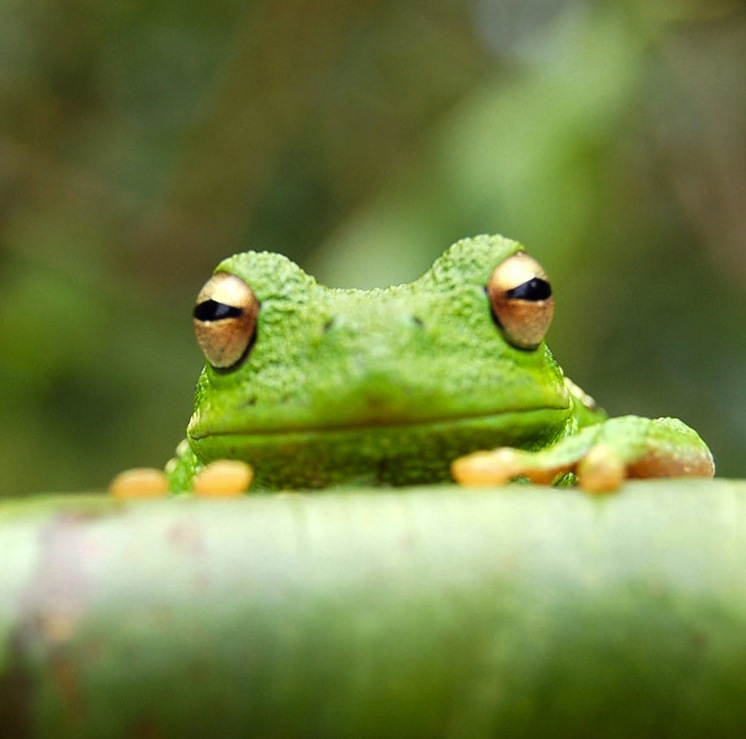
\includegraphics[width=0.5\textwidth]{frog.jpg}
%\caption{\label{fig:frog}This is a figure caption.}
%\end{figure}

\bibliography{example}
\end{document}
